% Graphics for slide 25, in the order the PDF draws them.
\begin{tikzpicture}[remember picture, overlay, x=1bp, y=-1bp,
  shift={(current page.north west)}]
\path[fill=cFFFFFF] (0,0) rectangle (960,540);
\node[anchor=north west, inner sep=0pt] at (56.69,477.21) {
\includegraphics[width=73.42bp, height=37.42bp]{figures/fundamentals-of-hpc/p03-1.png}};
\path[fill=cEE7628,even odd rule] (57.18,55.73) ..controls(57.96,55.73)and(58.6,56.37)..(58.6,57.15) --(58.6,85.5) ..controls(58.6,86.28)and(57.96,86.91)..(57.18,86.91) ..controls(56.4,86.91)and(55.76,86.28)..(55.76,85.5) --(55.76,57.15) ..controls(55.76,56.37)and(56.4,55.73)..(57.18,55.73);
\path[fill=cEE7628,even odd rule] (246.86,447.37) ..controls(246.86,438.65)and(253.93,431.58)..(262.65,431.58) --(697.35,431.58) ..controls(706.07,431.58)and(713.14,438.65)..(713.14,447.37) --(713.14,467.33) ..controls(713.14,476.05)and(706.07,483.12)..(697.35,483.12) --(262.65,483.12) ..controls(253.93,483.12)and(246.86,476.05)..(246.86,467.33) --(246.86,447.37);
\node[anchor=north west, inner sep=0pt] at (55.76,120.19) {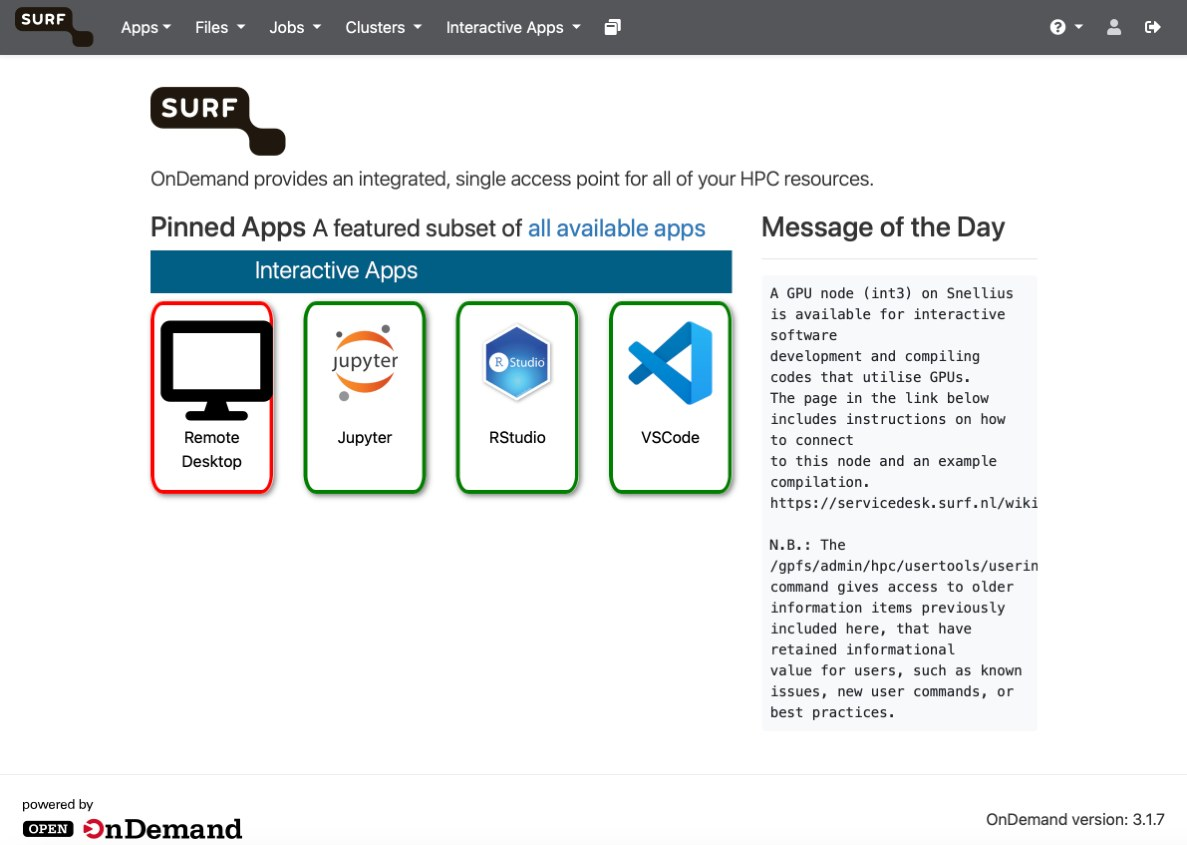
\includegraphics[width=395.43bp, height=281.22bp]{figures/fundamentals-of-hpc/p25-2.jpg}};
\end{tikzpicture}
